%!TEX root = ../thesis.tex
\chapter{Introduction}  % Main chapter title
\label{cha:introduction}

%----------------------------------------------------------------------------------------
%	SECTION 1
%----------------------------------------------------------------------------------------

\section{Main Section 1}


MR relation ship image arXiv:1506.05097~\citet{chen_probabilistic_2016}

\begin{figure}
    \centering
    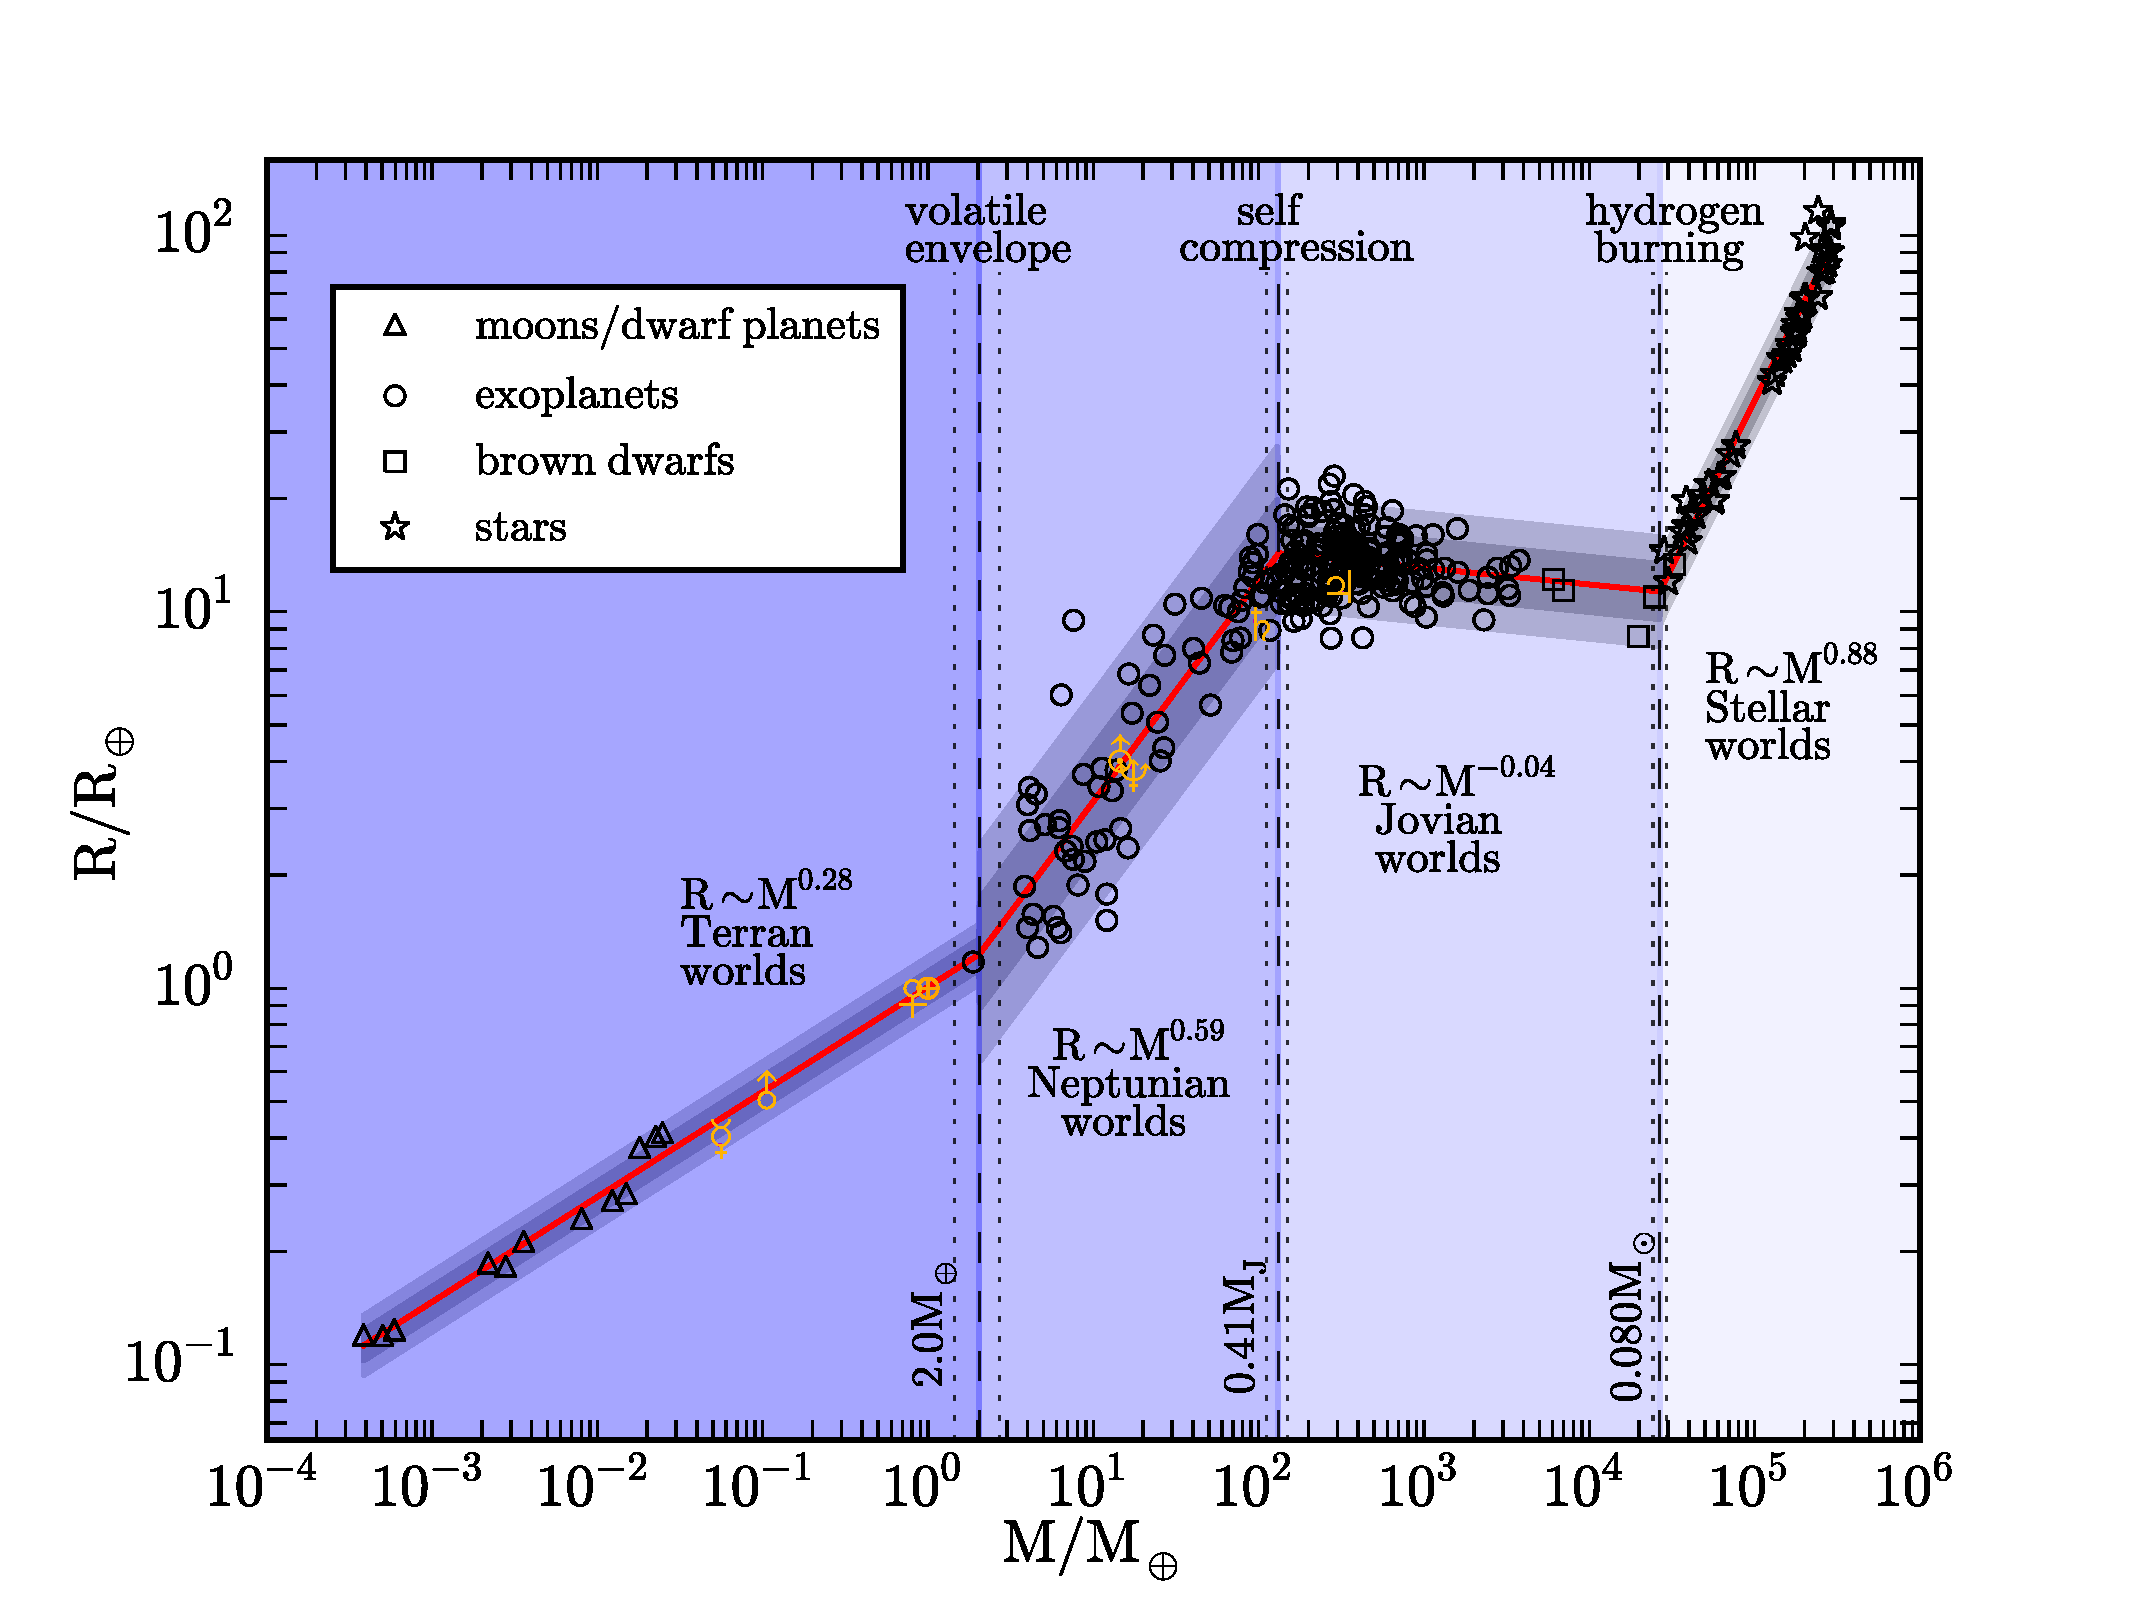
\includegraphics[width=0.7\linewidth]{./figures/introduction/plt_overlay_add.pdf}
    \caption{M-R relationship~\citet{chen_probabilistic_2016}}
    \label{fig:pltoverlayadd}
\end{figure}

Santos et al 2017 \todo{read and quote}

%-----------------------------------
%	SUBSECTION 1
%-----------------------------------
\subsection{Subsection 1}


%-----------------------------------
%	SUBSECTION 2
%-----------------------------------

\subsection{Subsection 2}

%----------------------------------------------------------------------------------------
%	SECTION 2
%----------------------------------------------------------------------------------------

\section{Main Section 2}


Spectral Disentangling techniques
- PSOAP
- Differencing Fruluga
- Templates ?


2D-cross-correlation?   piskorz 2016


\section{Recent detections in Companion spectra.}


Birkby


\subsection{model fitting transit stars (not actual title. more other similar methods)}
There are other situations in which to determine the presence of faint secondary spectra, such as, identifying the presence of any background or companion stars of transiting planet candidates. Many astronomical phenomena such as grazing eclipsing, a giant primary star eclipsed by a dwarf or a background star can produce signals indistinguishable from planetary transits. Efforts to characterize the false positive probability (FPP) among Kepler planet candidates is as high as $\sim35\%$~\citep{santerne_sophie_2012}. The presence of unknown companions or background stars decreases the dimming effect from the planet transit leading to smaller planetary radius. Where multiple stars are present there may also be ambiguity on which star hosts the planet.~\citet{kolbl_detection_2015} developed a method for detecting the presences of faint secondary lines in optical stellar spectra by matching observations to the SpecMatch library of stellar spectra. Identifying the spectroscopic evidence of a secondary star for 63/1160 California \emph{Kepler} Survey objects of Interest (KOI).


For transiting planets that presence of a background star or a companion star causes problems in characterizing the planet. Being able to detect spectra signal of the a faint second spectra in double-lined spectroscopic binaries.
For example eclipsing binaries,
A dim binary system companion or a gaint planet around a background star can mimic the transit of a small Earth-like planet on a foreground star.
